\documentclass{beamer}

% \usepackage{beamerthemesplit} // Activate for custom appearance

\title{Linear Algebra Review}
\author{Frank Wood}
%\date{\today}

\newcommand{\comment}[1]{}
\newcommand{\ponedec}{\mathcal{P}^\downarrow_1}
\newcommand{\pone}{\mathcal{P}_1}
\newcommand{\rank}[1]{\mathrm{RANK}\left[#1\right]}
\newcommand{\E}[1]{\mathrm{E}\left[#1\right]}
\newcommand{\py}{\mathcal{PY}}
\newcommand{\iid}{iid.}
\newcommand{\drawiid}{\stackrel{\text{iid}}{\sim}}
\newcommand{\vect}[1]{\mathbf{#1}}
\newcommand{\indicator}[1]{\text{I}\left[ #1 \right]}
\newcommand{\pdcoag}{PD(d_1,0)-\text{COAG}}
\newcommand{\todo}{\textbf{*TODO*}}
\newcommand{\igram}{\text{$\infty$-gram}}
\newcommand{\Prob}{\text{P}}

\def\mm{sequence memoizer }
\def\MM{SM }

\def\pibf{{\boldsymbol{\pi}}}
\def\kapbf{\boldsymbol{\kappa}}
\def\taubf{\boldsymbol{\tau}}
\def\thebf{\boldsymbol{\theta}}
\def\rhobf{\boldsymbol{\rho}}
\def\phibf{\boldsymbol{\phi}}
\def\pbf{\mathbf{p}}
\def\qbf{\mathbf{q}}
\def\sbf{\mathbf{s}}
\def\tbf{\mathbf{t}}
\def\ybf{\mathbf{y}}
\def\wbf{\mathbf{w}}
\def\xbf{\mathbf{x}}
\def\rbf{\mathbf{r}}
\def\tbf{\mathbf{t}}
\def\kbf{\mathbf{k}}
\def\Xbf{\mathbf{X}}
\def\0bf{\mathbf{0}}
\def\Ibf{\mathbf{I}}
\def\phibf{\mathbf{\phi}}
\def\Phibf{\mathbf{\Phi}}
\def\disteq{{\stackrel{D}{=}}}
\def\EE{{\mathbb{E}}}

\def\phiv{\varphi}
\def\phivbf{\boldsymbol{\varphi}}

\def\Ocal{\mathcal{O}}

\DeclareMathOperator*{\Bet}{Beta} \DeclareMathOperator{\coag}{COAG}
\DeclareMathOperator{\frag}{FRAG} \DeclareMathOperator*{\rnk}{RANK}
\DeclareMathOperator*{\gem}{GEM} \DeclareMathOperator*{\pd}{PD}
\DeclareMathOperator*{\gd}{GDir} \DeclareMathOperator*{\Dir}{Dir}
\DeclareMathOperator*{\Ave}{\mathbb{E}}
\DeclareMathOperator*{\Var}{Var}

\begin{document}

\frame{\titlepage}

%\section[Outline]{}
%\frame{\tableofcontents}
%
%\section{Introduction}
%\subsection{Overview of Topics}
%
%\section{Bayesian Analysis}
%\subsection{Single Parameter Model}
\frame[t] {
 \frametitle{Definition of Matrix}
 \begin{itemize}
 \item Rectangular array of elements arranged in rows and columns\\
 \[ \begin{bmatrix}
 16000 & 23\\
 33000 & 47\\
 21000 & 35
 \end{bmatrix} \]
\item A matrix has dimensions 
\item The dimension of a matrix is its number of rows and columns 
\item It is expressed as $3\times2$ (in this case)
 \end{itemize}
}

\frame[t] {
 \frametitle{Indexing a Matrix}
 \begin{itemize}
 \item Rectangular array of elements arranged in rows and columns\\
 \[ \bf A= \begin{bmatrix}
  a_{11} & a_{12} & a_{13}\\
 a_{21} & a_{22}& a_{23}\\
 \end{bmatrix} \]
\item A matrix can also be notated 
\[\mathbf{A}=[a_{ij}], a=1,2; j=1,2,3\]
 \end{itemize}
}

\frame[t] {
 \frametitle{Square Matrix and Column Vector}
 \begin{itemize}
 \item Square matrix has equal number of rows and columns\\
 \[ \begin{bmatrix}
 4 & 7\\
 3 & 9
 \end{bmatrix}~~~~~
 \begin{bmatrix}
  a_{11} & a_{12} & a_{13}\\
 a_{21} & a_{22}& a_{23}\\
 a_{31} & a_{32}& a_{33}
 \end{bmatrix} \]
\item A column vector is a matrix with a single column\\
 \[ \begin{bmatrix}
 4 \\
 7\\
 10
 \end{bmatrix}~~~~~
 \begin{bmatrix}
c_1\\
c_2\\
c_3\\
c_4\\
c_5\\
 \end{bmatrix} \]
 \item All vectors (row or column) are matrices, all scalars are $1\times1$ matrices.
 \end{itemize}
}


\frame[t] {
 \frametitle{Transpose}
 \begin{itemize}
 \item The transpose of ta matrix is another matrix in which the rows and columns have been interchanged\\
 \[ \bf A= \begin{bmatrix}
2 & 5 \\
 7 &10\\
 3& 4
 \end{bmatrix} \]\\
 \[ \bf A'= \begin{bmatrix}
2 & 7 & 3 \\
 5 & 10 & 4\\
 \end{bmatrix} \]
 \end{itemize}
}

\frame[t] {
 \frametitle{Row Vector}
 \begin{itemize}
 \item A row vector is the transpose of a column vector or a matrix with a single row\\
 \[ \bf B= \begin{bmatrix}
 15 & 25 & 50
 \end{bmatrix} ~~~~~
 \bf F'= \begin{bmatrix}
f_1 & f_2
 \end{bmatrix}\]
 \end{itemize}
}

\frame[t] {
 \frametitle{Equality of Matrices}
 \begin{itemize}
 \item Two matrices are the same if they have the same dimension and all the elements are equal\\
 \[ \bf A= \begin{bmatrix}
 a_1\\
 a_2\\
 a_3
 \end{bmatrix} ~~~~~
 \bf B= \begin{bmatrix}
4\\
7\\
3
 \end{bmatrix}\]
 $A=B$ implies $a_1=4, a_2=7, a_3=3$
 \end{itemize}
}

\frame[t] {
 \frametitle{Regression Examples}
 \[ \bf Y= \begin{bmatrix}
Y_1\\
Y_2\\
.\\
.\\
.\\
Y_n
\end{bmatrix} \]
}

\frame[t] {
 \frametitle{Regression Examples}
 Design matrix\\
 \[ \bf X= \begin{bmatrix}
 1 & X_1\\
 1 & X_2\\
.\\
.\\
.\\
1  &X_n
\end{bmatrix} \]
}

\frame[t] {
 \frametitle{Matrix Addition and Substraction}
 \[ \bf A= \begin{bmatrix}
1&4\\2&5\\3&6
 \end{bmatrix}~~~~
 \bf B= \begin{bmatrix}
 1 &2\\ 2 &3\\ 3 &4\\
 \end{bmatrix} \]
 Then
 \[
 \bf A+B= \begin{bmatrix}
2 &6\\ 4&8\\ 6&10
 \end{bmatrix}\]
}

\frame[t] {
 \frametitle{Regression Example}
 $Y_i=E(Y_i)+\epsilon_i,\;i=1,...,n$\\
 \[
 E(\bf Y)= \begin{bmatrix}
E(Y_1)\\
E(Y_2)\\
.\\
.\\
.\\
E(Y_n)\\
\end{bmatrix}~~~
\bf \epsilon= \begin{bmatrix}
\epsilon_1\\
\epsilon_2\\
.\\
.\\
.\\
\epsilon_n\\
\end{bmatrix}
 \]
 \[
\begin{bmatrix}
Y_1\\
Y_2\\
.\\
.\\
.\\
Y_n
\end{bmatrix}=\begin{bmatrix}
E(Y_1)\\
E(Y_2)\\
.\\
.\\
.\\
E(Y_n)\\
\end{bmatrix}+\begin{bmatrix}
\epsilon_1\\
\epsilon_2\\
.\\
.\\
.\\
\epsilon_n\\
\end{bmatrix}=\begin{bmatrix}
E(Y_1)+\epsilon_1\\
E(Y_2)+\epsilon_2\\
.\\
.\\
.\\
E(Y_n)+\epsilon_n\\
\end{bmatrix}
 \]
}

\frame[t] {
 \frametitle{Multiplication of a Matrix by a Scalar}
 \[
 \bf {A}= \begin{bmatrix}
 2& 7\\
 9&3
 \end{bmatrix}\]
 \[  k \mathbf{A} = k \begin{bmatrix}
 2& 7\\
 9&3
 \end{bmatrix}=\begin{bmatrix}
 2k& 7k\\
 9k&3k
 \end{bmatrix}\]
}

\frame[t] {
 \frametitle{Multiplication of two Matrices}
 \begin{figure}[h!]
   \centering
    % \caption{}
     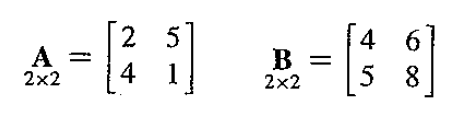
\includegraphics[scale=.3]{13_1.png}
 \end{figure}\begin{figure}[h!]
   \centering
    % \caption{}
     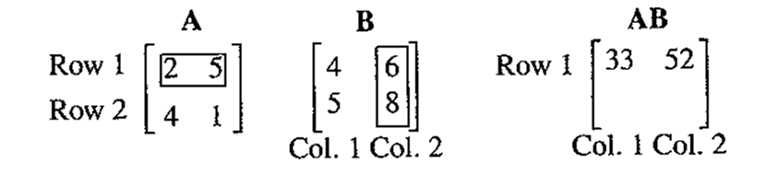
\includegraphics[scale=.3]{13.png}
 \end{figure}
\begin{figure}[h!]
   \centering
    % \caption{}
     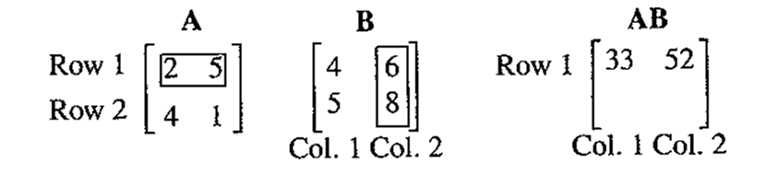
\includegraphics[scale=.3]{13_3.png}
 \end{figure}
}

\frame[t] {
 \frametitle{Another Matrix Multiplication Example}
\[ \bf A= \begin{bmatrix}
1& 3 &4\\0&5&8
\end{bmatrix}~~~~~~
\bf B= \begin{bmatrix} 3\\5\\2
\end{bmatrix} \]
\[ \bf AB= \begin{bmatrix}
1& 3 &4\\0&5&8
\end{bmatrix}
\begin{bmatrix} 3\\5\\2
\end{bmatrix}=
\begin{bmatrix}
26\\41
\end{bmatrix}
\]
}

\frame[t] {
 \frametitle{Regression Example}
 \[ \begin{bmatrix}
1 &X_1\\
1 &X_2\\
1 &X_3\\
 \end{bmatrix}
\begin{bmatrix}
\beta_0\\
\beta_1
\end{bmatrix}=\begin{bmatrix}
\beta_0+\beta_1 X_1\\
\beta_0+\beta_1 X_2\\
\beta_0+\beta_1 X_3\\
\end{bmatrix} \]

}

\frame[t]  {
 \frametitle{Regression example}
 Sum of squares
 \begin{eqnarray*} \bf Y'Y &=& \bf Y'IY\\
  &=& \begin{bmatrix}
 Y_1 & Y_1 &...&Y_n
\end{bmatrix}
\begin{bmatrix}
Y_1\\
Y_2\\
.\\
.\\
.\\
Y_n\\
\end{bmatrix}\\
&=&\begin{bmatrix}
Y_1^2+Y_2^2+...+Y_n^2
\end{bmatrix}\\&=&\begin{bmatrix}
\sum Y_i^2
\end{bmatrix} \end{eqnarray*}

}

\frame[t]  {
 \frametitle{More Regression Examples}

\[ \bf X'X= \begin{bmatrix}
1&1&...&1\\
 X_1 & X_1 &...&X_n
\end{bmatrix}
\begin{bmatrix}
1&X_1\\
1&X_2\\
.\\
.\\
.\\
1&X_n
\end{bmatrix}=\begin{bmatrix}
n&\sum X_i\\
\sum X_i & \sum X_i^2
\end{bmatrix} \]

\[ \bf X'Y= \begin{bmatrix}
1&1&...&1\\
 X_1 & X_1 &...&X_n
\end{bmatrix}
\begin{bmatrix}
Y_1\\
Y_2\\
.\\
.\\
.\\
Y_n\\
\end{bmatrix}=\begin{bmatrix}
\sum Y_i\\
\sum X_i Y_i
\end{bmatrix} \]
}

\frame[t] {
 \frametitle{Special Matrices}
 \begin{itemize}
 \item If $A=A'$, then A is a symmetric matrix
 \[\bf A= \begin{bmatrix}
 1&4&6\\
 4&2&5\\
 6&5&3
 \end{bmatrix}~~~~~
 \bf A'=\begin{bmatrix}
 1&4&6\\
 4&2&5\\
 6&5&3
 \end{bmatrix} \]
 \item If the off-diagonal elements of a matrix are all zeros it is
 then called a diagonal matrix
 \[\bf A= \begin{bmatrix}
 a_1 &0&0\\
 0&a_2&0\\
 0&0&a_3
 \end{bmatrix}~~~~~
 \bf B=\begin{bmatrix}
 4 &0&0&0\\
 0&1&0&0\\
 0&0&10&0\\
 0&0&0&5
 \end{bmatrix}\]
 \end{itemize}

}

\frame[t] {
 \frametitle{Identity Matrix}
 A diagonal matrix whose diagonal entries are all ones is an
 identity matrix. Multiplication by an identity matrix leaves the pre
 or post multiplied matrix unchanged.
\[  \bf I=\begin{bmatrix}
 1 &0&0&0\\
 0&1&0&0\\
 0&0&10&0\\
 0&0&0&1
 \end{bmatrix}\]
 and
 \[ \bf AI = IA = A\]

}

\frame[t] {
 \frametitle{Vector and matrix with all elements equal to one}
\[ \bf 1= \begin{bmatrix}
1\\
1\\
.\\
.\\
.\\
1
\end{bmatrix}~~~~
\bf J= \begin{bmatrix}
1 &...&1\\
.&.&.\\
.&.&.\\
.&.&.\\
1 &...&1
\end{bmatrix}\] 

\[\bf 1 1'=\begin{bmatrix}
1\\
1\\
.\\
.\\
.\\
1
\end{bmatrix}\begin{bmatrix}
1&
1&
.&
.&
.&
1
\end{bmatrix}=\begin{bmatrix}
1 &...&1\\
.&.&.\\
.&.&.\\
.&.&.\\
1 &...&1
\end{bmatrix}=J\]
}
\frame[t] {
 \frametitle{Linear Dependence and Rank of Matrix}
 Consider\\
 \[ \bf A= \begin{bmatrix}
 1&2&5&1\\
 2&2&10&6\\
 3&4&15&1
 \end{bmatrix} \]
 and think of this as a matrix of a collection of column vectors.
 \bigskip
 
 Note that the third column vector is a multiple of the first column
 vector.
}

\frame[t] {
 \frametitle{Linear Dependence}
 When $c$ scalars $k_1,...,k_c$ not all zero, can be found such
 that:
 \begin{center}
 $k_1 C_1+...+k_c C_c=0$
 \end{center}
 where 0 denotes the zero column vector and $C_i$ is the $i^{th}$ column of matrix $C$, the $c$ column vectors are called
 linearly dependent. If the only set of scalars for which the
 equality holds is $k_1=0,...,k_c=0$, the set of c column vectors is
 linearly independent.\\
 \bigskip
 
 In the previous example matrix the columns are linearly dependent.
 \[ 5\begin{bmatrix}
 1\\2\\3
 \end{bmatrix}+0\begin{bmatrix}
 2\\2\\4
 \end{bmatrix}-1\begin{bmatrix}
 5\\10\\15
 \end{bmatrix}+0\begin{bmatrix}
 1\\6\\1
 \end{bmatrix}=\begin{bmatrix}
 0\\0\\0
 \end{bmatrix}\]
}

\frame[t] {
 \frametitle{Rank of Matrix}
 The rank of a matrix is defined to be the maximum number of
 linearly independent columns in the matrix.  Rank properties include
\begin{itemize}
\item  The rank of a matrix is unique\\
\item  The rank of a matrix can equivalently be defined as the maximum number of linearly
 independent rows\\
\item  The rank of an $r\times c$ matrix cannot exceed $min(r,c)$
\item The row and column rank of a matrix are equal
\item The rank of a matrix is preserved under nonsingular transformations., i.e. Let $\bf A$ $(n\times n)$ and $\bf C$ $(k\times k)$ be nonsingular matrices.  Then for any $n \times k$ matrix $\bf B$ we have
\[ rank(\mathbf{B}) = rank(\mathbf{AB}) = rank (\bf BC)\]
\end{itemize}

}


\frame[t] {
 \frametitle{Inverse of Matrix}
 \begin{itemize}
 \item Like a reciprocal \\
 \[6*1/6=1/6*6=1\]
 \[x\frac{1}{x}=1\]
 \item But for matrices\\
 \[\bf AA^{-1}=A^{-1}A=I\]
 \end{itemize}
}

\frame[t] {
 \frametitle{Example}
 \[ \bf A= \begin{bmatrix}
 2 &4 \\
 3 &1
 \end{bmatrix}\]\\
 \[ \bf{A} ^{-1}=\begin{bmatrix}
-.1 & .4\\
.3 &-.2
 \end{bmatrix}\]
 \[ \bf A^{-1}A=\begin{bmatrix}
1&0\\
0&1
 \end{bmatrix}\]
}

\frame[t] {
 \frametitle{Inverses of Diagonal Matrices are Easy}
 \[ \bf A= \begin{bmatrix}
 3&0&0\\
 0&4&0\\
 0&0&2
 \end{bmatrix}\]
}

\frame[t] {
 \frametitle{Relation of Rank and Inverse}
 \begin{itemize}
 \item An inverse of a square $r\times r$ matrix exists if the rank of the
 matrix is $r$.
 \item Such a matrix is said to be nonsingular (or full rank)
 \item An $r\times r$ matrix with rank less than $r$ is said to be singular
 and does not have an inverse
 \item The inverse of an $r \times r$ matrix of full rank also has rank $r$
 \end{itemize}
}

\frame[t] {
 \frametitle{Finding the inverse}
 \begin{itemize}
 \item Finding an inverse takes (for general matrices with no special structure)
 \begin{center}
 $O(n^3)$
 \end{center}
 operations (when n is the number of rows in the matrix)
 \item We will assume that numerical packages can do this for us
 \end{itemize}
}

\frame[t] {
 \frametitle{Manual Inverse Finding}
 \begin{itemize}
 \item For small matrices it is possible to find an analytical
 matrix inverse
 \item Example
 \begin{center}
 \[ \bf{X'X}= \begin{bmatrix}
 n & \sum X_i\\
 \sum X_i & \sum X_i^2
 \end{bmatrix} \]\\
 \[ (\bf{X'X})^{-1}= \begin{bmatrix}
 \frac{1}{n}+\frac{\bar{X}}{\sum(X_i-\bar{X})^2} &
 \frac{-\bar{X}}{\sum(X_i-\bar{X})^2}\\
 \frac{-\bar{X}}{\sum(X_i-\bar{X})^2} & \frac{1}{\sum(X_i-\bar{X})^2}
 \end{bmatrix}
 \]
 \end{center}
 \end{itemize}
}

\frame[t] {
 \frametitle{Uses of Inverse Matrix}
 \begin{itemize}
 \item Ordinary algebra $5y=20$\\
 is solved by $1/5*(5y)=1/5*(20)$
 \item Linear algebra $\bf AY=C$\\
 is solved by $\mathbf{A}^{-1}\mathbf{AY=A}^{-1}\mathbf{C, Y=A}^{-1}\mathbf{C}$
 \end{itemize}

}

\frame[t] {
 \frametitle{Example}
 Solving a system of simultaneous equations\\
 \begin{center}
 $2y_1+4y_2=20$\\
 $3y_1+y_2=10$
 \[ \begin{bmatrix}
 2&4\\
 3&1
 \end{bmatrix} \begin{bmatrix}
 y_1\\
 y_2
 \end{bmatrix}=\begin{bmatrix}
 20\\
 10
 \end{bmatrix} \]
  \[ \begin{bmatrix}
 y_1\\
 y_2
 \end{bmatrix}= \begin{bmatrix}
 2 &4\\
 3 &1
 \end{bmatrix}^{-1}\begin{bmatrix}
 20\\
 10
 \end{bmatrix} \]
 \end{center}
}

\frame[t] {
 \frametitle{List of Useful Matrix Properties}
 \begin{eqnarray*}
 \bf A+B&=& \bf B+A\\
  \bf (A+B)+C&=& \bf A+(B+C)\\
  \bf (AB)C&=& \bf A(BC)\\
  \bf C(A+B)&=& \bf CA+CB\\
 k(\bf A+B)&=&k\mathbf{A}+k\mathbf{B}\\
 \bf (A')'&=& \bf A\\
  \bf (A+B)'&=& \bf A'+B'\\
  \bf (AB)'&=& \bf B'A'\\
  \bf (ABC)'&=& \bf C'B'A'\\
  (\mathbf{AB})^{-1}&=&\mathbf{B}^{-1}\mathbf{A}^{-1}\\
 (\mathbf{ABC})^{-1}&=&\mathbf{C}^{-1}\mathbf{B}^{-1}\mathbf{A}^{-1}\\
 (\mathbf{A}^{-1})^{-1}&=&\mathbf{A}\\
 (\mathbf{A}')^{-1}&=&(\mathbf{A}^{-1})'
 \end{eqnarray*}
}

\frame[t] {
 \frametitle{Derivatives}
 \begin{eqnarray*}
 \bf A+B&=& \bf B+A\\
  \bf (A+B)+C&=& \bf A+(B+C)\\
  \bf (AB)C&=& \bf A(BC)\\
  \bf C(A+B)&=& \bf CA+CB\\
 k(\bf A+B)&=&k\mathbf{A}+k\mathbf{B}\\
 \bf (A')'&=& \bf A\\
  \bf (A+B)'&=& \bf A'+B'\\
  \bf (AB)'&=& \bf B'A'\\
  \bf (ABC)'&=& \bf C'B'A'\\
  (\mathbf{AB})^{-1}&=&\mathbf{B}^{-1}\mathbf{A}^{-1}\\
 (\mathbf{ABC})^{-1}&=&\mathbf{C}^{-1}\mathbf{B}^{-1}\mathbf{A}^{-1}\\
 (\mathbf{A}^{-1})^{-1}&=&\mathbf{A}\\
 (\mathbf{A}')^{-1}&=&(\mathbf{A}^{-1})'
 \end{eqnarray*}
}










\end{document}
